%%%
%% v3.3 [2020/05/14]
%\documentclass[Proof,technicalreport]{ieicej}
\documentclass[technicalreport]{ieicej}
\usepackage{graphicx}
%\usepackage[fleqn]{amsmath}
%\usepackage{amsthm}
%\usepackage{amssymb}
\usepackage{latexsym}
\usepackage{newtxtext}
\usepackage[varg]{newtxmath}
\usepackage{url}
\usepackage{amsmath}
\usepackage{autobreak}

\def\IEICEJcls{\texttt{ieicej.cls}}
\def\IEICEJver{3.2}
\newcommand{\AmSLaTeX}{%
 $\mathcal A$\lower.4ex\hbox{$\!\mathcal M\!$}$\mathcal S$-\LaTeX}
%\newcommand{\PS}{{\scshape Post\-Script}}
\def\BibTeX{{\rmfamily B\kern-.05em{\scshape i\kern-.025em b}\kern-.08em
 T\kern-.1667em\lower.7ex\hbox{E}\kern-.125em X}}

\jtitle{交差点における建物遮蔽とリンク状態を考慮した地理的opportunistic routing}
\etitle{(SIGO)Building Shadowing on Intersection and Link State aware Geographic Opportunistic Routing for Urban VANETs }
% \esubtitle{Guide to the Technical Report and Template}
\authorlist{%
 \authorentry[hanako@denshi.ac.jp]{高橋 柊人}{Shuto Takahashi}{BKC}% 
 \authorentry[taro@jouhou.co.jp]{吉田 政望}{Masami Yoshida}{BKC}% 
 \authorentry[jiro@jouhou.co.jp]{ガジェゴス ラモネト アルベルト}{Alberto Gallegos Ramonet}{gakubu}% 
 \authorentry[jiro@jouhou.co.jp]{野口 拓}{Taku Noguchi}{gakubu}%
}
\affiliate[BKC]{立命館大学情報理工学研究科\hskip1zw
  〒522-8577 滋賀県草津市野路東1-1-1}
 {Graduate School of Information Science and Engineering, Ritsumeikan University\hskip1em
  1-1-1 Noji-h-gashi, Kusatsu, Shiga 525-8577, Japan}
\affiliate[gakubu]{立命館大学情報理工学部\hskip1zw
  〒522-8577 滋賀県草津市野路東1-1-1}
 {Graduate School of Information Science, 
  Ritsumeikan University\hskip1em
  1-1-1 Noji-h-gashi, Kusatsu, Shiga 525-8577, Japan}

% \MailAddress{$\dagger$is0361er@ed.ritsumei.ac.jp,
% $\dagger\dagger$\{taro,jiro\}@ritsumei.ac.jp}

\MailAddress{$\dagger$is0361er@ed.ritsumei.ac.jp,$\dagger$is0195hr@ed.ritsumei.ac.jp,$\dagger\dagger$ramonet@fc.ritsumei.ac.jp,$\dagger\dagger$noguchi@ed.ritsumei.ac.jp
}


\begin{document}
\begin{jabstract}
 複雑な都市環境での車両アドホックネットワーク(VANETs)では, 建物や樹木などの障害物が多数存在するため, シャドウイングやフェージングが起こり, 電波伝搬の妨害が発生する. しかし, 多くの既存Opportunistic Routing Protocolの性能評価では, シミュレーションでシャドウイングの影響が考慮されておらず, 通信性能が過大評価されている可能性がある. そこで, 本研究では、既存routing protocolの性能評価をネットワークシミュレータNS3のシャドウイングモデルであるObstacle Modelを用いた場合の、通信性能への影響を調査し, 新たにシャドウイングを考慮した交差点ベースのprotocol(SIGO)を提案する. SIGOは中継ノードの優先度を決める指標として, 中継ノードと目的地までの距離, 中継ノードとの予想伝送確率に加えて, 交差点の中継ノードが優先的に選択される指標を追加した. シミュレーションにより, パケット到達率の向上と, エンドツーエンド遅延の減少を確認し, SIGOの通信性能の有効性を示した. 
\end{jabstract}
\begin{jkeyword}
VANET,Opportunistic routing, シャドウイング
\end{jkeyword}
\begin{eabstract}
In complex urban ad hoc networks (VANETs), many obstacles such as buildings and trees can cause shadowing and fading, which can interfere with the propagation of radio waves. However, many existing opportunistic routing protocols do not take the shadowing effect into account, which may lead to overestimation of the performance. In this study, we investigate the performance of existing routing protocols by using the Obstacle Model of the NS3 network simulator to evaluate the performance of existing protocols, and newly propose an intersection-based protocol (SIGO) is proposed. In addition to the distance to the destination and the transmission probability, SIGO adds a node preference for the nodes at the intersection as a relay node selection metric. The simulation results show that the packet arrival rate is improved, the overhead is reduced, and the effectiveness of the communication performance is demonstrated.
\end{eabstract}
\begin{ekeyword}
p\LaTeXe\ class file, typesetting
\end{ekeyword}
\maketitle

\section{まえがき}


自動車運転の安全性や利便性の向上, 環境負担の低減を目的とし, 高度交通システム(Intelligent Transportations System : ITS) \cite{ITS} に関する取り組みが盛んにおこなわれている. 車車間通信を利用して形成される車両アドホックネットワーク(Vehicle Ad Hoc Networks: VANETs) は, ITSにおける多様なアプリケーションの実現に必要不可欠である. VANETsでは, 無線通信機を搭載した車車間でアドホック通信を行うことで、リアルタイム性と柔軟性を持つネットワーク構築が可能となる. しかし,  ITSシステムを安定してサポートするためには, 通信オーバーヘッドの削減, 高いパケット到達率, リアルタイム性を実現するrouting protocolが必要となる. \par
 都市環境での車両ネットワークでは, ノードのモビリティや建物の存在を考慮する必要があり, 典型的なrouting手法\cite{Old1},\cite{Old2}では, ノードの高速なモビリティへの対応が課題とされている[4]. これらの手法に対して, opportunistic routingが注目を集めている\cite{EXOR}. opportunistic routingと従来のroutingの最大の違いは, 固定ルートを使用せず, パケットを受信した車両が再転送するか否かを自己選択する点である. これにより, 従来のrouting方式に比べて, opportunistic routingは中継パケットを受信する機会を増やし, 結果として優れたパフォーマンスを実現できることを示している.\par
 しかし, 既存のopportunistic routing protocolの多くは,都市環境を想定して考案されているが, 性能評価で建物によるシャドウイングの影響が考慮されておらず,通信性能を過大評価している可能性がある.
 
 そこで本研究では, 既存opportunistic routing protocolであるLSGO protocol\cite{LSGO}をネットワークシミュレータns-3のシャドウイングモデルであるObstacle Model\cite{Obstacle}を用いて評価し, 建物によるシャドウイングが起こる場合と起こらない場合とでの通信性能を評価する. また, シャドウイングが起こる環境での通信性能の向上を目的としたSIGO protocolを提案する. SIGOは中継ノード選択する指標として, 目的地までの距離, 伝送確率に加えて, 交差点のノードが優先的に選択される指標を追加した. 提案手法の有効性をシャドウイングが考慮されたシミュレーション環境で評価する.\par
 2章では既存opportunistic routing protocolを紹介し課題点を述べ, 3章では提案手法について紹介し, 4章ではシミュレーションでLSGO protocolのシャドウイングが起こる場合の通信性能への影響の評価と, 提案手法の有効性について示す. 最後に5章でまとめと今後の課題について述べる.


\section{関連研究}

近年, opportunistic routing protocolが注目を集めている. これは従来のgeographic routing \cite{GPSR}\cite{GPCR}などに比べ, 中継ノードがパケット受信する機会を増やすことで通信性能の向上を果たしている. opportunistic routingの基本モデルを図\ref{fig:Basic}に示す.ノード$N_{i}$が送信ノード, $N_{d}$が宛先ノードである. 送信ノードNsは中継候補ノードとして, $N_{1}$ ~ $N_{n}$を選択し, 選択したノードそれぞれに優先順位を指定してパケットを送信する. 受信した$N_{1}$ ~ $N_{n}$のノードはそれぞれ自身の優先順位を確認し, 優先順位の高いノードから再転送を行う. また, 各中継ノードは自身より優先度の高いノードの再転送を受信すると自身の再転送をキャンセルし, 冗長なパケットの増加を防いでいる. これらのことから, opportunistic routingにおいて, 優先度の選択アルゴリズムが通信性能に直接影響を及ぼすことがわかる.\par
代表的なopportunistic routing としてEXOR\cite{EXOR}が提案されている. これは, 中継ノードの優先度選択アルゴリズムとして, ETX\cite{ETX}とは似ているが異なる独自の予想伝送コストを計算し, 優先度を決める指標となっている. しかし, この新たに考案されたETX値は, VANETの性質であるノードのランダムで高速なモビリティを考慮していないという問題がある.\par
そこで, 新たにVANETに適したETX値を考案したLSGO\cite{LSGO}が提案された. LSGOでは, 予想伝送コストと呼ばれるVANET用に最適化されたETX値を, 優先度を決定する指標として使用し, パケット到達率の向上, エンドツーエンド遅延の減少を実現しいる. また, SCAOR\cite{SCAOR}では, パケットの衝突でネットワークのパフォーマンスを低下させる問題を防ぐために, ノード密度パラメータを, 優先度決定における指標として追加し, LSGOやEXORに比べ通信性能が向上したことを示している.\par
 しかし, これらのprotocol に共通する課題として, シミュレーションの性能評価として, 建物によるシャドウイングが考慮されていないことが挙げられる. この問題によりこれらのprotocol は通信性能を過大評価している可能性がある. 本研究では, LSGO protocol について, シミュレーションを用いて, シャドウイングを考慮した場合の通信性能への影響を調査し, シャドウイングを考慮したrouting手法に焦点を当てる.
 \begin{figure}[!ht]
\centering
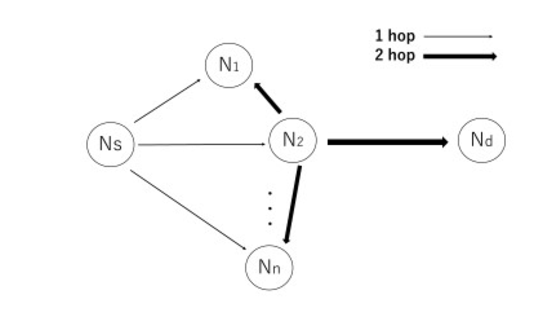
\includegraphics[width=90mm]{figures/basic-opportunity.eps}
\caption{opportunistic routingの基本モデル}
\label{fig:Basic}
\end{figure}



\section{提案手法}
本研究では, 中継ノードを選択し, 優先度を決定するための指標として, 目的地までの進度( 送信車両に比べてどれだけ目的地に近いか), リンク状態, 交差点度数の3つの指標を用いたSIGOを提案する. 
\subsection{リンクの品質の推定}
SIGOでは, 各ノードがHelloパケットを定期的にブロードキャストし, それを用いてリンク状態ETXを推定する. Helloパケットは, 自ノードのID, X座標, Y座標で構成されている. ETXを算出するために, 各ノードは近隣ノードから最初にHelloパケットを受信した時間$t_{0}$を記録する. そして, 現在時刻を$t$, ウィンドウサイズを$w$(second), Helloパケットの送信間隔を$τ$とすると, 予想伝送確率$r(t)$はウィンドウサイズ$w$で場合分けされ, 式1で算出される.
\begin{equation}
r(t) =\begin{cases}count(t, t_{0}), & 0 < t - t_{0} < 1,  \\ \frac{count(t,t_{0})}{(t-t_{0}) / τ}, & 1 \leq t - t_{0} \leq w\\
\frac{count(t - w,t)}{w / τ}, &  t - t_{0} \geq w\\
\end{cases}
\end{equation}

$(t,t_{0})$ / $τ$は, ウィンドウサイズの間に受信されるべきHelloパケット数であり, $count(t,t_{0})$は$t$ ~ $t_{0}$の期間中に実際に受信されたHello パケットの数である. \par
 各近隣車両とのリンクの非対称性は考慮せず, 一方向の予想伝送確率$r_{t}$のみを使用してETXを計算する. 一方向伝送確率が$r_{t}$であると仮定すると, リンクETXは式(2)で算出される.
 
 \begin{equation}
 ETX = \frac{1}{r^{2}(t)} 
 \end{equation}

\subsection{交差点度数}
SIGOでは, 建物によるシャドウイングの影響を最小限にするため, 交差点ノードが優先的に中継ノードとして選択される指標を追加する. 交差点度数は以下の式(3)で算出される.

\begin{equation}
 交差点度数 = αθ
 \end{equation}
 
  θは送信車両と 宛先車両を結ぶ直線と,送信車両と交差点車両を結ぶ直線のなす角である(図\ref{fig:Intersection}). 
  $θ$が大きくなるほど, 交差点度数は大きくなり, 後述する優先度決定アルゴリズムにより交差点ノードが優先される可能性が増加する. $α$は, 交差点度数の重み付けであり, この値が増加するほど交差点度数が増加し, 交差点ノードが優先される確率が増加する. 
 
 \begin{figure}[!ht]
\centering
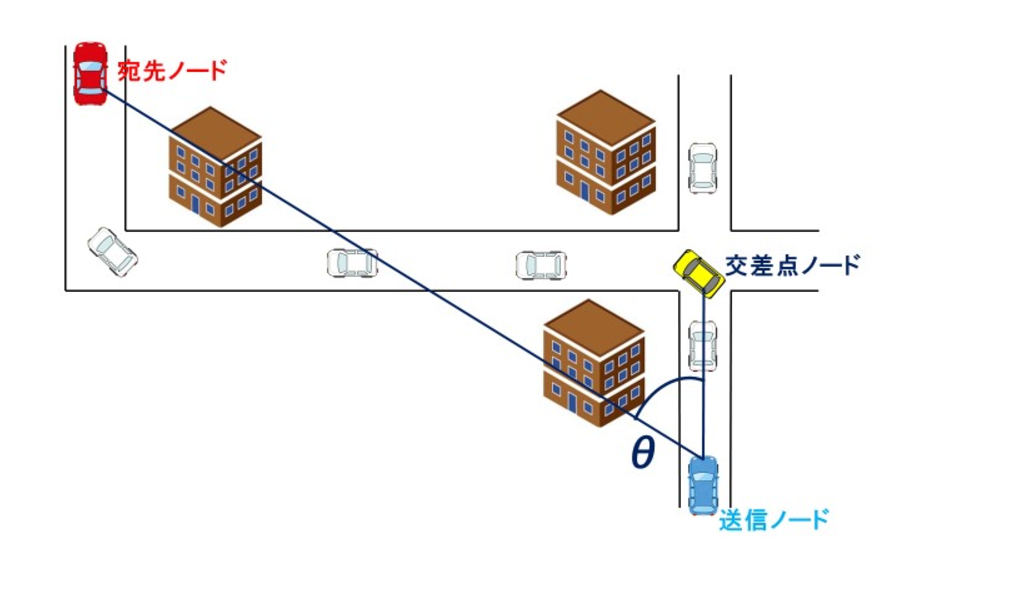
\includegraphics[width=90mm]{figures/Intersection.eps}
\caption{交差点度数}
\label{fig:Intersection}
\end{figure}

\subsection{候補ノード選択アルゴリズム}
SIGOは, 信頼性を確保しながら, 送信回数を減らすため最適な個数かつ最適なノードを候補ノードとして選択する必要がある. 候補ノード数を$N$とすると, $N$は次の条件を満たす必要がある. 
\begin{equation}
1 - \prod_{i=0}^n (1 - r_{i}(t))\geq R
\end{equation}

\begin{eqnarray}
d_{1}(t) \times αθ \leq   d_{2}(t) \times αθ \leq   d_{i}(t)  \times αθ  \leq \nonumber \\ 
d_{i}(t) \times αθ   \leq  d_{N}(t)  \times αθ \left(αθは交差点ノードのみ\right)
\end{eqnarray}

\begin{equation}d_{i}(t) < s_{i}(t)
\end{equation}
式(4)における$r_{i}(t)$ (1$ \leqq $i$ \leqq $N)は, 送信車両が保持する隣接車両との予想伝送確率である. 式(6)における$d_{i}(t)$は隣接車両$i$から目的地までの距離, $S_{t}(t)$は送信車両から目的地までの距離である. 
式(4)の左辺は送信車両からのパケットを候補ノード1~$N$のいずれかの車両が受信すると予想される確率であり, 右辺$R$は単一リンクに必要な伝送確率である. 車両密度が小さい場合や送信者車両と各隣接車両との予想伝送確率が低い場合, 式(4)満たすことができない場合がある. その場合, 式(6)を満たすすべての隣接車両が候補車両として選択される. また, 送信車両と各隣接車両との予想伝送確率が高い場合, 候補ノード数$N$は小さくなるため, 信頼性を確保しながら, 最低限の候補ノード数を選択することができる. 
\subsection{優先度スケジューリングアルゴリズム}
SIGOでは, タイマーベースの優先度スケジューリングアルゴリズムを使用する. このアルゴリズムでは, 最も優先度が高いノードが最初にパケットを送信する. ほかの候補ノードは, 優先順位の高いノードからのパケットを受信すると, 自身のパケットを破棄する. タイマーが期限切れになり, 自身より優先度の高いノードからのパケットを受信していない場合, 送信を開始する. SIGOは以下の式(7)(8)によって, 優先度が決定される.

\begin{equation}
\frac{D_{sd} - D{id}}{ETX_{i}^{2}} \times αθ
\end{equation}

\begin{equation}
\frac{D_{sd} - D{id}}{ETX_{i}^{2}} 
\end{equation}

$D_{sd}$は送信車両から目的地までの距離, $D_{id}$は候補車両$i $から目的地までの距離である. 式(7)は交差点車両, 式(8)は交差点以外に位置する車両に適用される.

\section{性能評価}
性能評価では, ネットワークシミュレータNs-3[12]と交通流シミュレータSUMO[13] を用いて評価を行う. また, シャドウイングの影響をシミュレーションで考慮させるため, 電波減衰モデルとしてObstacle shadowing model [7]を用いた. 4.2節でシャドウイングによる電波減衰がシミュレーションで評価される場合とされない場合とでの通信性能の違いを評価し, 4.3節でSIGO protocol の性能評価を行う.

\subsection{シミュレーション設定}
シミュレーションパラメータを表\ref{tab:parameter}, シミュレーションシナリオを図\ref{fig:scenario}に示す. シミュレーション開始時に, ランダムな送信ノードと宛先ノードがそれぞれ20台ずつ割り当てられ, 通信を開始する. 
\begin{table}[!ht]
\begin{center}
\caption{シミュレーションパラメータ}
\label{tab:parameter}
\begin{tabular}{|l|l|lll}
\cline{1-2}
Simulation area    & 2100m × 2100m   &  &  &  \\ \cline{1-2}
Mobility model     & Random mobility &  &  &  \\ \cline{1-2}
Transmission range & 250m            &  &  &  \\ \cline{1-2}
Number of vehicles & 400 ~ 1000      &  &  &  \\ \cline{1-2}
\end{tabular}
\end{center}
\end{table}

\begin{figure}[!ht]
\centering
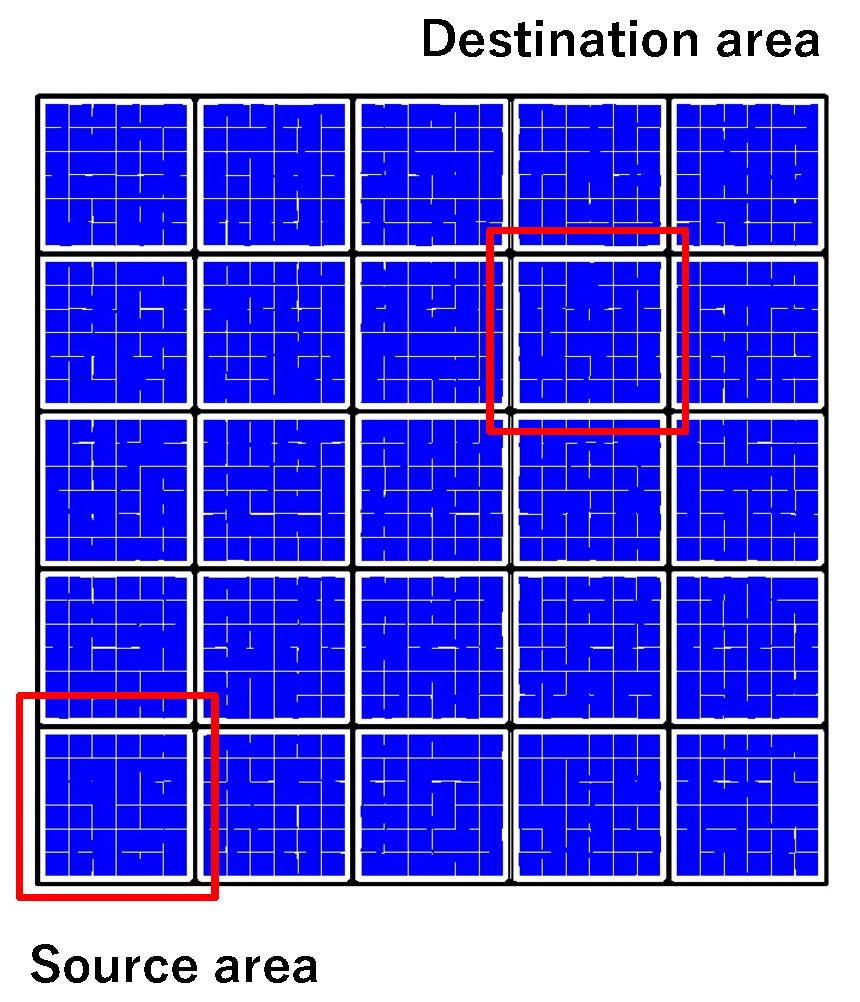
\includegraphics[width=90mm]{figures/scenario.eps}
\caption{シミュレーションシナリオ}
\label{fig:scenario}
\end{figure}

\par

\subsection{シャドウイングの影響}
シミュレーションで建物のシャドウイングによる電波の減衰が起こる場合,  LSGO protocolの通信性能に与える影響をパケット到達率, エンドツーエンド遅延, オーバーヘッドの3つの評価項目で評価した. 
図\ref{fig:PDR-shadowing}はネットワークシミュレータでシャドウイングの影響を考慮した場合としない場合とでの, パケット到達率を示している. パケット到達率は, 送信ノードが送信した合計パケット数に対する, 宛先ノードが受信したパケット数の合計の比率である. 図\ref{fig:PDR-shadowing}では, シミュレーションでシャドウイングを考慮した場合, 全てのノード数においてパケット到達率が減少している. これは, シャドウイングによる電波減衰が原因だと推測される.

\begin{figure}[!ht]
\centering
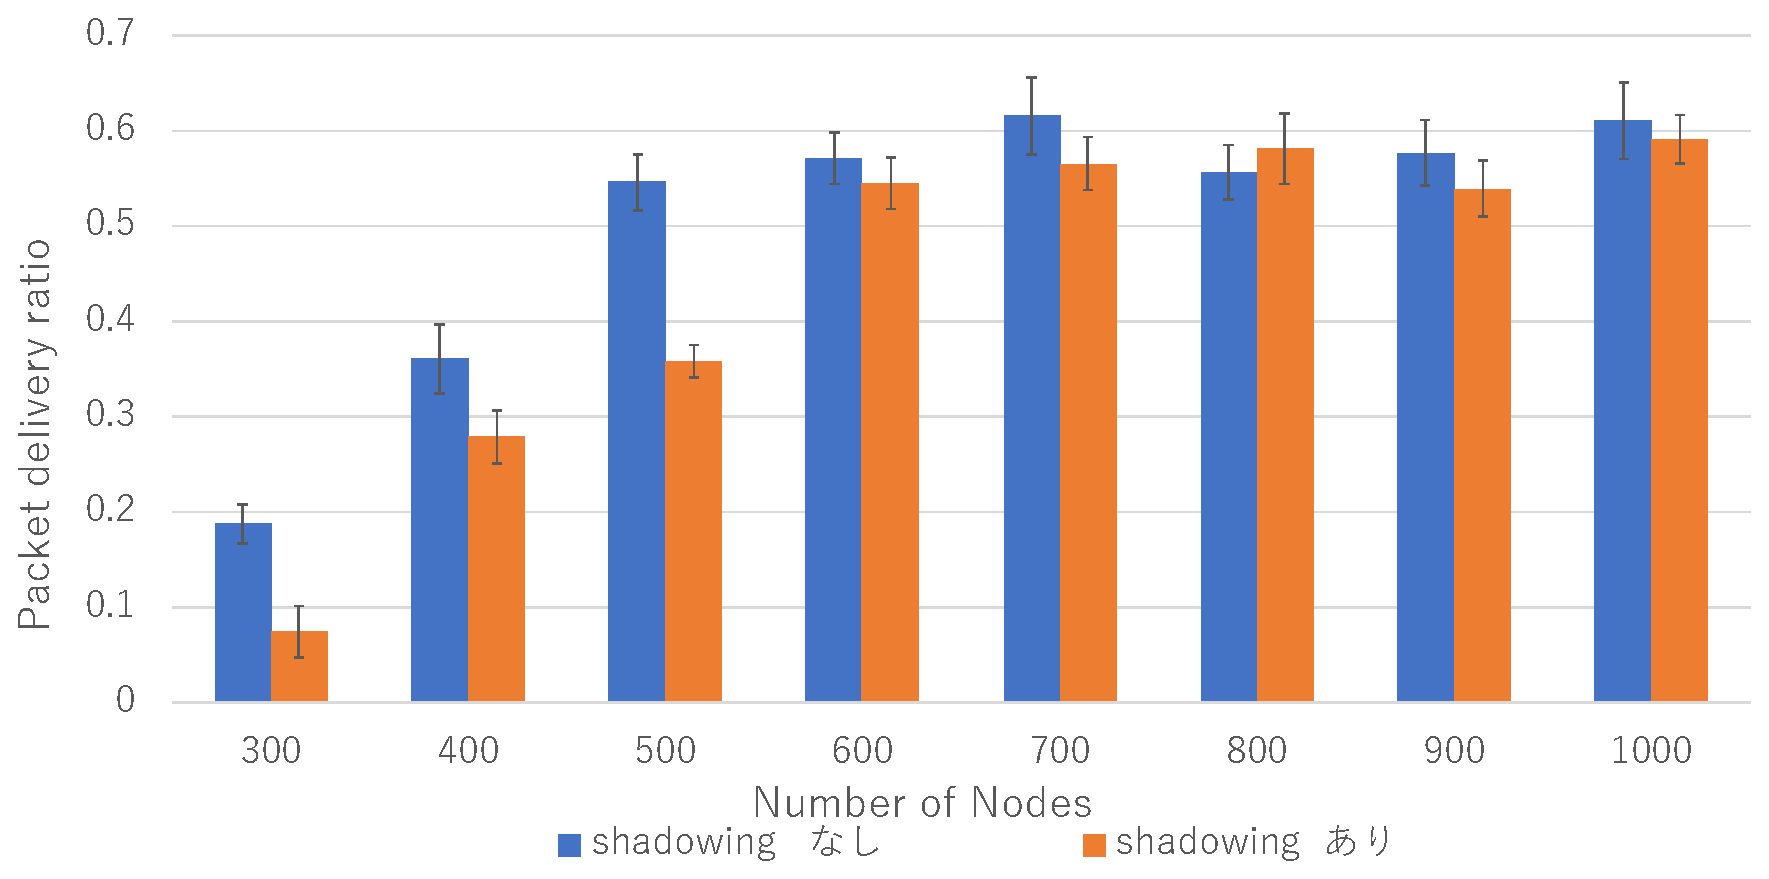
\includegraphics[width=90mm]{figures/PDR-shadowing.eps}
\caption{パケット到達率 シャドウイングの有無}
\label{fig:PDR-shadowing}
\end{figure}

図\ref{fig:Delay-shadowing}はネットワークシミュレータでシャドウイングの影響を考慮する場合としない場合とでのエンドツーエンド遅延を示している. エンドツーエンドの遅延は送信ノードがパケットを送信してから宛先ノードが正常に受信するまでにかかる平均時間として定義する. 図\ref{fig:Delay-shadowing}では, シミュレーションでシャドウイングを考慮した場合, 全てのノード数においてエンドツーエンド遅延が増加している. これはシャドウイングによる電波減衰が起こり, 建物を通過するパケットが届きにくくなることで, 送信ノードと宛先ノードを直線的に結ぶような経路が形成することが難しくなったことが原因だと考えられる. 

\begin{figure}[!ht]
\centering
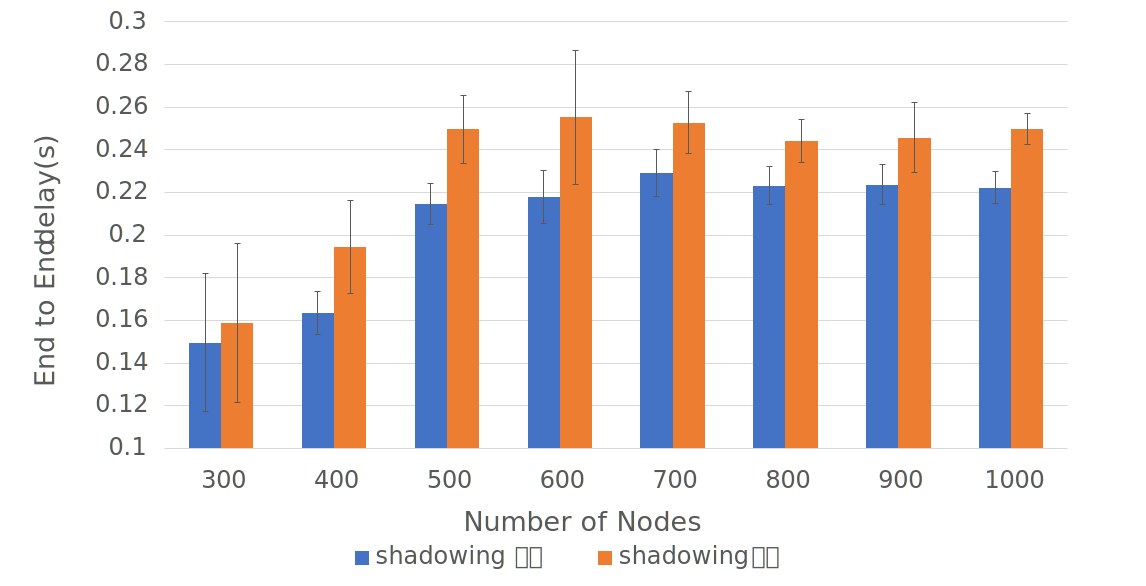
\includegraphics[width=90mm]{figures/Delay-shadowing.eps}
\caption{エンドツーエンド遅延 シャドウイングの有無}
\label{fig:Delay-shadowing}
\end{figure}


図\ref{fig:Overhead-shadowing}はネットワークシミュレータでシャドウイングの影響を考慮した場合としない場合とでの, オーバーヘッドを示している. (※オーバーヘッドはパケットの総数?)これは, opportunistic routing での送信ノードから指定された候補ノード同士が自分より優先度の高いノードからのパケットを建物による電波減衰によって, 受け取れない確率が増加しているからだと推測される. 


\begin{figure}[!ht]
\centering
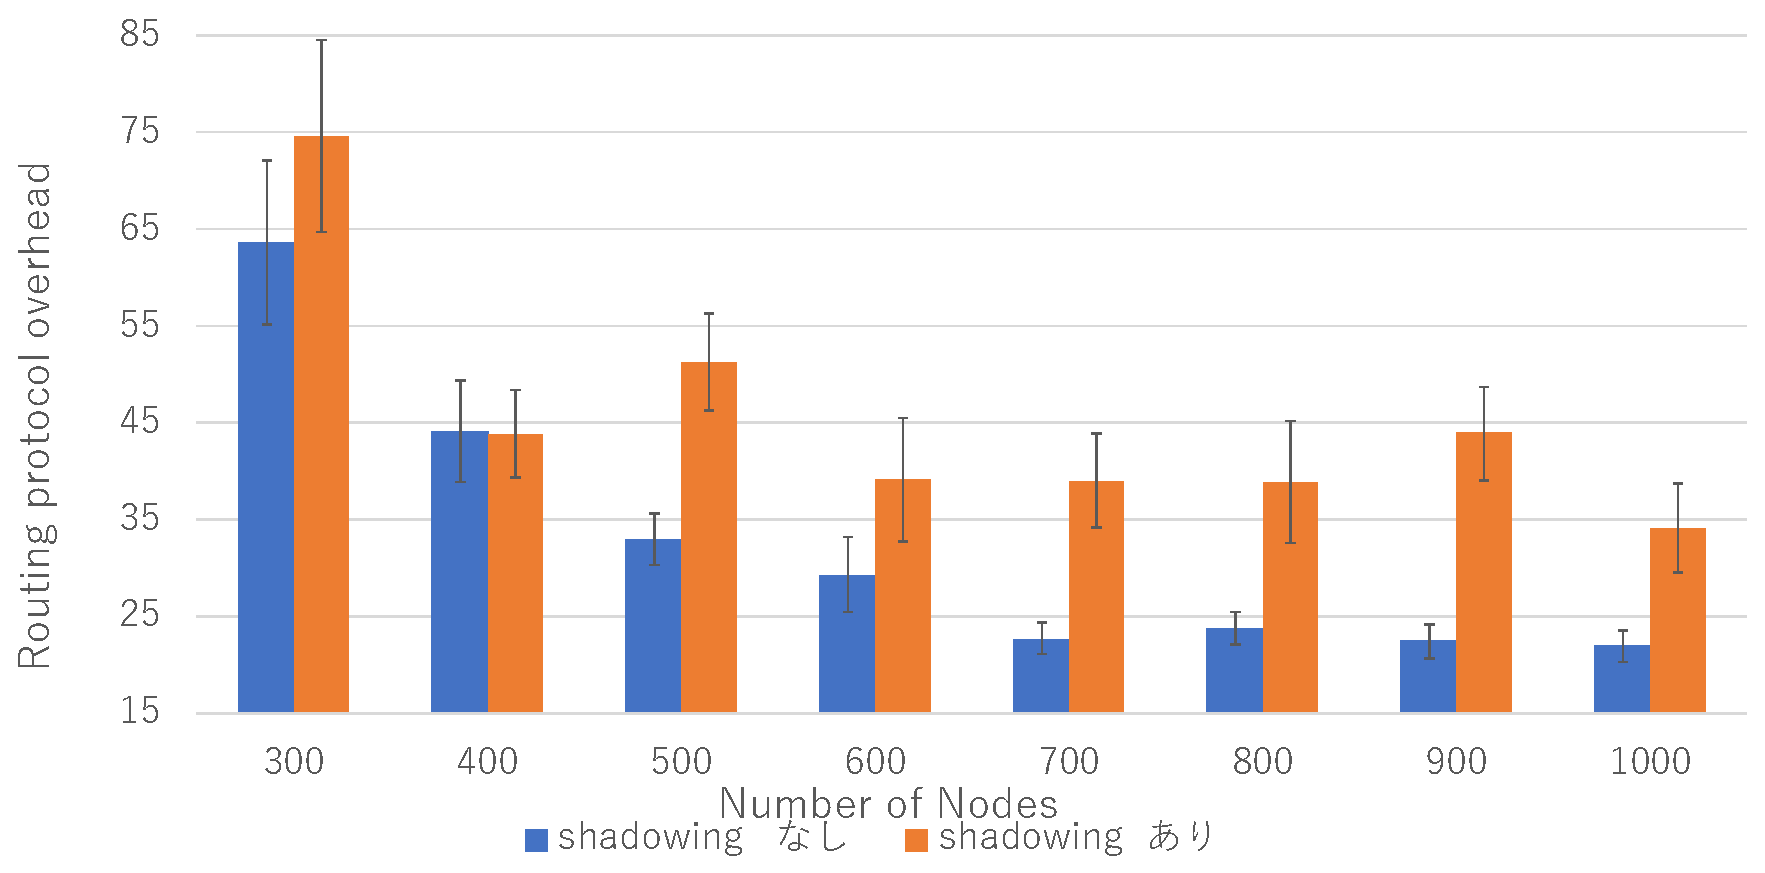
\includegraphics[width=90mm]{figures/Overhead-shadowing.eps}
\caption{オーバーヘッド シャドウイングの有無}
\label{fig:Overhead-shadowing}
\end{figure}


\subsection{SIGOの評価}
提案手法の有用性を評価するために, 4.2章と同様にパケット到達率, エンドツーエンド遅延, オーバーヘッドの3つの評価項目でLSGO protocolとの比較を行った. (※建物が多いシナリオと少ないシナリオの定義のようなものを記述できませんか?)

図\ref{fig:PDR}は建物が多い場合と, 建物が少ない場合でのSIGOとLSGOのパケット到達率を示している. 図\ref{fig:PDR}では, 建物が多いシナリオでは, SIGOはLSGOに比べてパケット到達率の向上していることがわかる. これはSIGOでは, 交差点ノードの優先度が高くなる可能性が高まり, よりシャドウイングの影響を受けにくいルートが形成することができているからだと推測される. 
一方, 建物が少ないシナリオではSIGOはLSGOに比べてパケット到達率の安定した向上は得られなかった. これは, シャドウイングの影響が少ないシナリオでは, 交差点ノードを優先させる利点が少なかったことが原因として推測される. 

\begin{figure}[!ht]
\centering
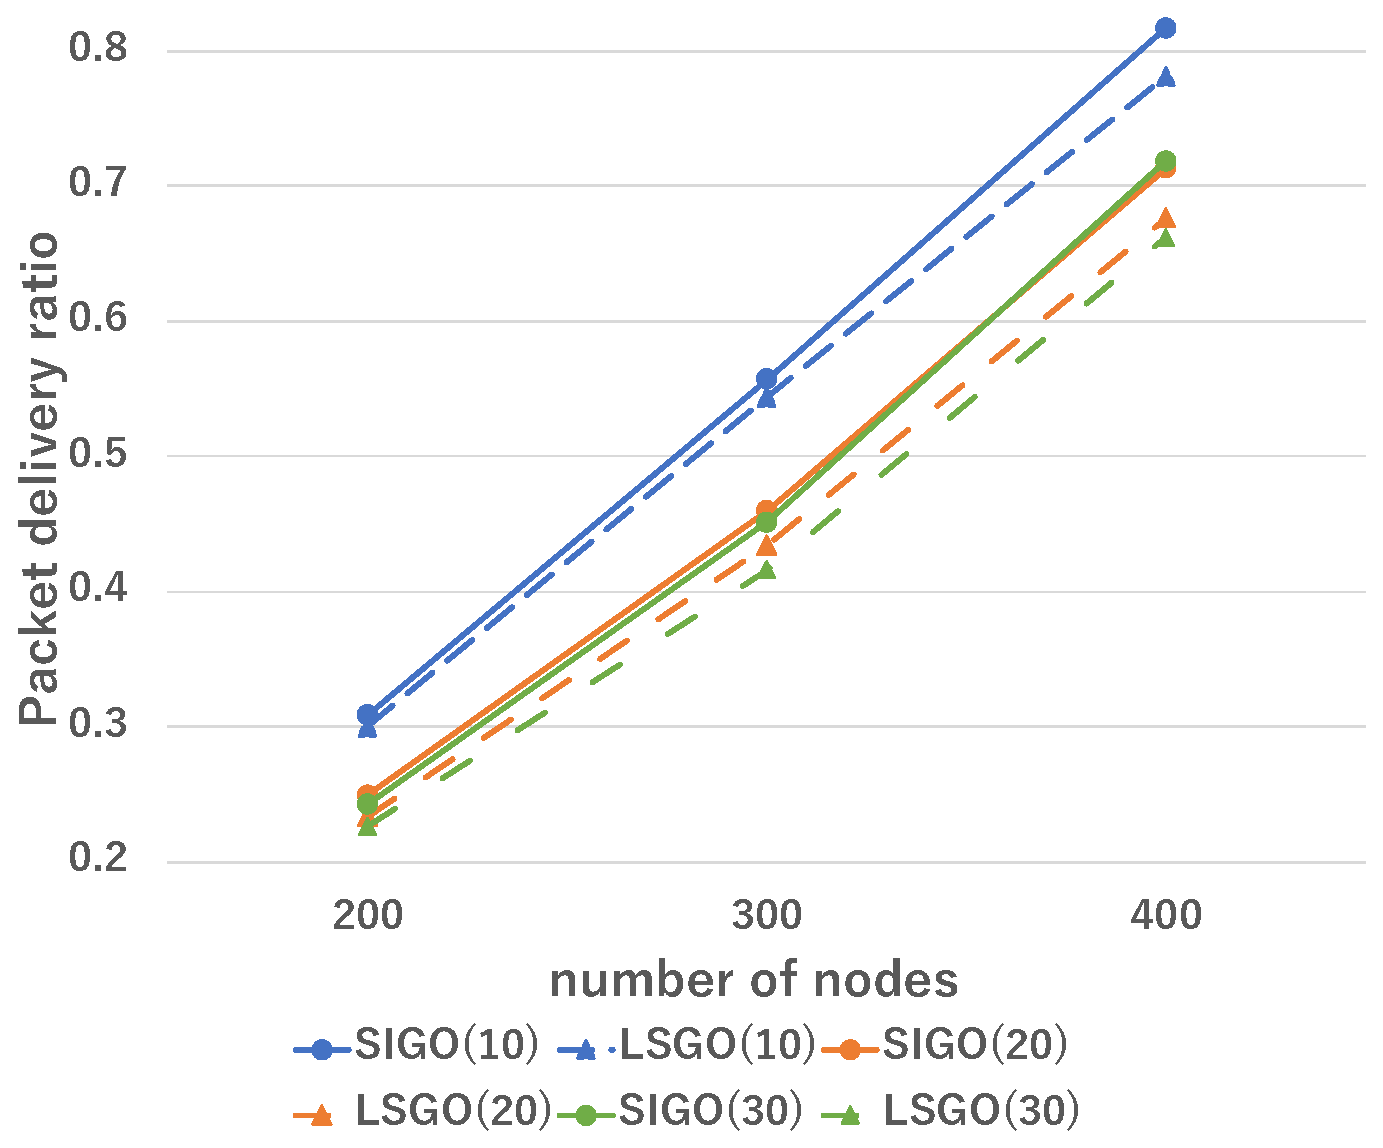
\includegraphics[width=90mm]{figures/PDR.eps}
\caption{パケット到達率 LSGO vs SIGO}
\label{fig:PDR}
\end{figure}


 図\ref{fig:Delay}は建物が多い場合と, 建物が少ない場合でのSIGOとLSGOエンドツーエンド遅延を示している. 建物が多い場合は, SIGOはLSGOに比べてエンドツーエンドの遅延が減少していることがわかる. これは, 交差点ノードの優先度が高くなる可能性が高まり, よりシャドウイングの影響を受けにくく, 候補ノードへパケットが正常に伝搬される可能性が高まることで, 優先度が高く, 待ち時間が短いノードがパケットを中継している確率が高いことが原因だと推測される. 一方, シャドウイングの影響が少ないシナリオでは, LSGOに比べて遅延が増加していることがわかる. これは交差点ノードがシャドウイングの影響が少ないにもかかわらず優先され, ホップ数が増加していることが原因として推測される. 
 
 \begin{figure}[!ht]
\centering
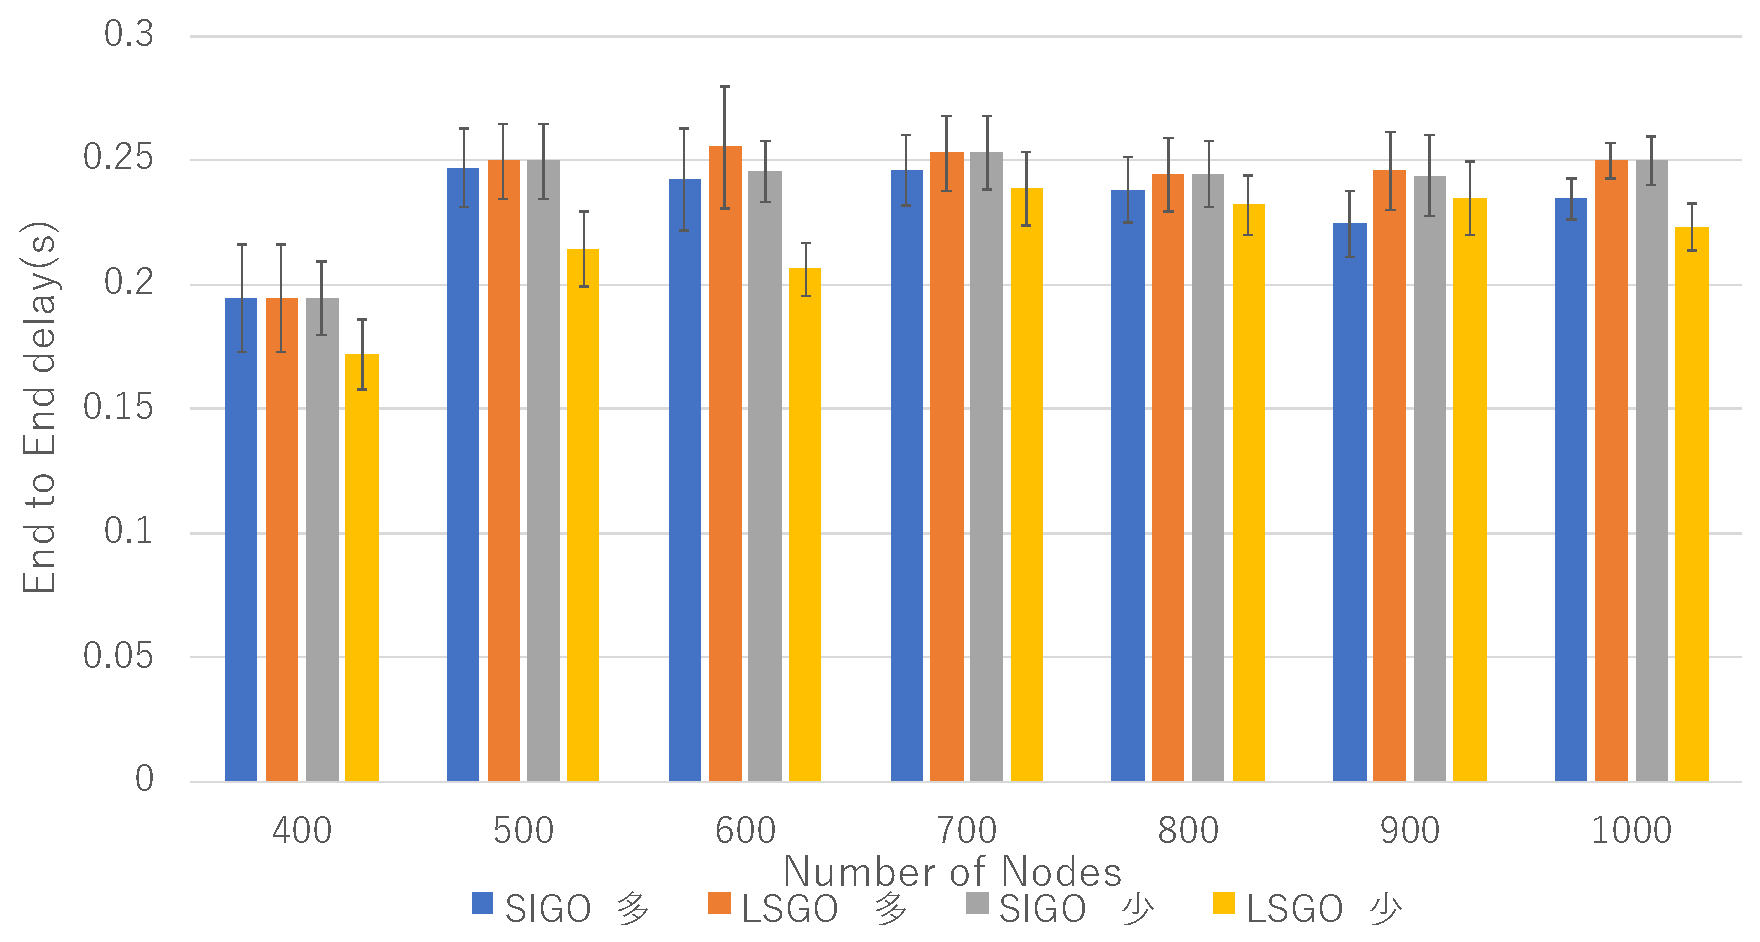
\includegraphics[width=90mm]{figures/Delay.eps}
\caption{エンドツーエンド遅延 LSGO vs SIGO}
\label{fig:Delay}
\end{figure}

図\ref{fig:Overhead}は建物が多い場合と, 建物が少ない場合でのSIGOとLSGOのオーバーヘッドを示している. SIGOはLSGOに比べて建物が多いときと少ないとき, どちらの場合もオーバーヘッドが増加してしまっていることがわかる. これはLSGOに比べてSIGOでは交差点ノードが優先される確率が高く, 比較的道に沿ってパケットが中継されるため, ホップ数が増加したと推測される. また, 図2のように交差点ノードが候補ノードとして異なる道路に位置する選択する可能性が高まり, 優先順位の高い候補ノードからのパケットをシャドウイングの影響で受け取れない可能性が増加することで冗長なパケットが増加したことが原因だと推測される(※この意味が理解しにくいです). 

 \begin{figure}[!ht]
\centering
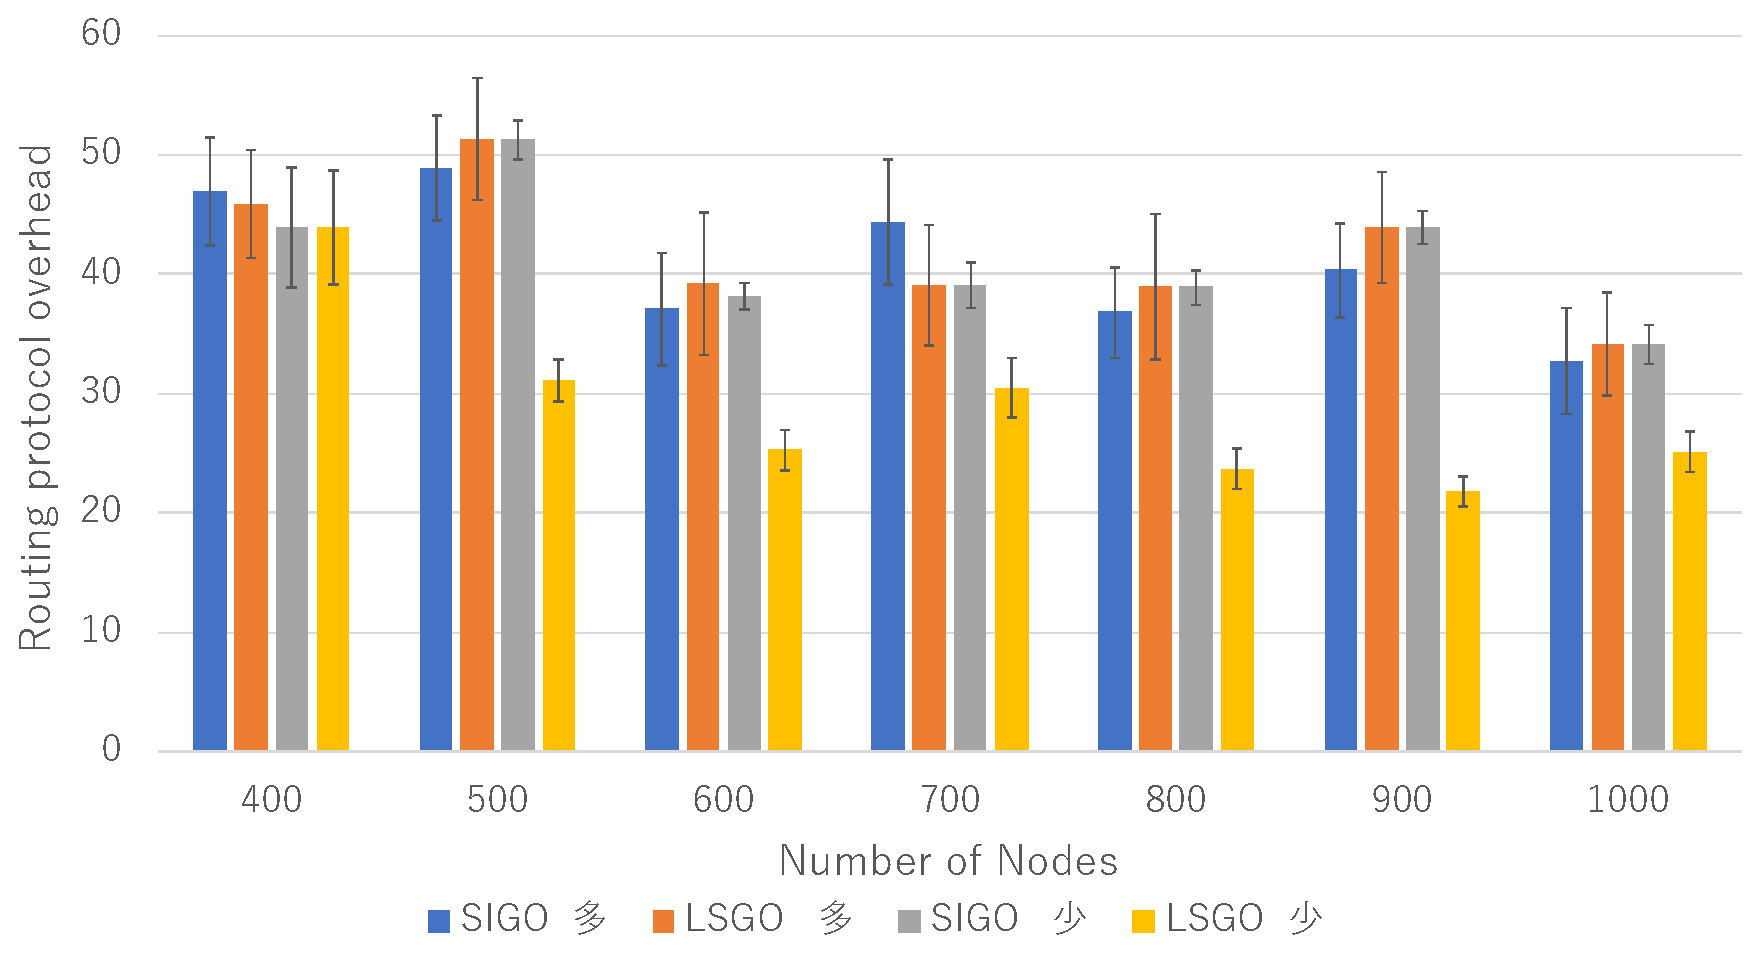
\includegraphics[width=90mm]{figures/Overhead.eps}
\caption{オーバーヘッド LSGO vs SIGO}
\label{fig:Overhead}
\end{figure}





\section{まとめ}
本研究では, 既存opportunistic routing protocolがシミュレーションでシャドウイングに対する影響を評価できていない問題, またそれによってrouting protocolを設計するにあたってシャドウイングの影響を考慮できていないという問題に着目し,シミュレーションでシャドウイングを考慮した評価を行った. 既存routing protocolはシミュレーションでシャドウイングに対する影響を評価した場合, 通信性能が低下することを示した. また, シャドウイングの影響を受けにくいルートを形成するSIGOを提案し, パケット到達率の向上, エンドツーエンド遅延の減少を確認し, 有効性を示した. しかし, 建物が少なくシャドウイングが起こりにくいシナリオでは既存 routing protocolと比較して, エンドツーエンド遅延, オーバーヘッドが増加する可能性が高いという傾向がみられた. 今後は, ノードの優先度を求めるだけでなく道路の優先度を決定することで冗長なパケットを防ぐことや, Hello パケットの情報を利用し, シャドウイングの影響の大きさを推測し, 交差点度数の重みづけαを固定値ではなく, 可変値するなどの対策が必要だと考える. 




\begin{thebibliography}{99}
% \bibitem{A}IBM セキュアなIoTソリューションの設計と構築
% \url{https://www.ibm.com/developerworks/jp/iot/library/iot-trs-secure-iot-solutions2/index.html}
% \bibitem{B}吉田耕太, 西村浩二, 大東俊博, 相原玲二 : 秘密分散法を利用したクラウドストレージサービスにおけるモバイル機器を考慮した安全な処理委託方式 情報処理学会論文誌, Vol.55, No.3, pp.1117-1125(Mar. 2014)
% \bibitem{C}Javier Munster, Hans-Arno Jacobsen : Secret Sharing in Pub/Sub Using Trusted Execution Enviroments, DEBS'18, June 25-29, 2018
% \bibitem{D}松尾正克, 古賀田勝則, 田中裕之, 武藤浩二, 小林正明 : IoT機器のための暗号・認証技術, およびサイバー攻撃検知, 対策技術, Panasonic Technical Journal, Vol.64, No.1, May 2018
% \bibitem{E}木村一統, 新井イスマイル, 藤川和利 : MQTT-SNの実装評価, 「

\bibitem{ITS}	国土交通省道路局:ITS スポット(オンライン),入手先
\url{http://www.mlit.go.jp/road/ITS/j-html/spot dsrc/ index.html}
\bibitem{Old1}Lochert, C., Mauve, M., Fussler, H. and Hartenstein, H.: Geographic Routing in City Scenarios, ACM SIGMO- BILE Mobile Computing and Communications Review, Vol.9, No.1, pp.69–72 (2005).
\bibitem{Old2}	H. Tong, Nonlinear Time Series: A Dynamical System Approach, J. B. Elsner, ed., Oxford University Press, Oxford, 1990.
\bibitem{EXOR}	S Biswas, R Morris, ExOR: opportunistic multi-hop routing for wireless networks, in Proceedings of the 2005 Conference on Applications, Technologies, Architectures, and Protocols for Computer Communications, Philadelphia, August 2005, pp. 133–144 
\bibitem{LSGO} 	uelian Cai, Ying He, Chunchun Zhao, Lina Zhu, and Changle Li.Lsgo: Link state aware geographic opportunistic routing protocolfor vanets.EURASIP Journal on Wireless Communications andNetworking, Vol. 2014, No. 1, p. 96, Jun 2014.
\bibitem{Obstacle} 	S. E. Carpenter and M. L. Sichitiu, “An obstacle model implementa- tion for evaluating radio shadowing with ns-3,” in Proc. WNS, 2015, pp. 17–24.
\bibitem{GPSR} 	B Karp, HT Kung, GPSR: greedy perimeter stateless routing for wireless networks, in Proceedings of Mobile Computing and Net-working, Boston, August 2000, pp. 243–254.
\bibitem{GPCR}	C Lochert, M Mauve, H Füssler, H Hartenstein, Geographic routing in city scenarios, in Proceedings of the SIGMOBILE Mobile Computing and Communications Review, vol. 9(1), 2005, pp. 69–72.
\bibitem{ETX} DSJ De Couto, D Aguayo, J Bicket, R Morris, A high throughput path metric for multi-hop wireless routing, in Proceedings of the 9th Annual International Conference on Mobile Computing and Networking (MobiCom’ 03), San Diego, September 2003, pp. 134–146.
\bibitem{SCAOR}Sadatpour, V, Zargari, F Ghanbari, M. A Collision Aware Opportunistic Routing Protocol for VANETs in Highways. Wireless Pers Commun 109, 175–188 (2019).
\bibitem{NS3} Network Simulator ns3https://www.nsnam.org
\bibitem{SUMO} Simulation of Urban Mobility https://sumo.dlr.de/docs/index.html 
\end{thebibliography}



\end{document}
